\documentclass[tikz,border=7pt]{standalone}
\usepackage{amsmath}
\usetikzlibrary{positioning,arrows.meta,fit}
\tikzset{
  box/.style={draw,rectangle,rounded corners=2pt,minimum width=52mm,minimum height=28mm,align=left},
  arr/.style={-{Latex[length=2mm]},thick}
}
\begin{document}
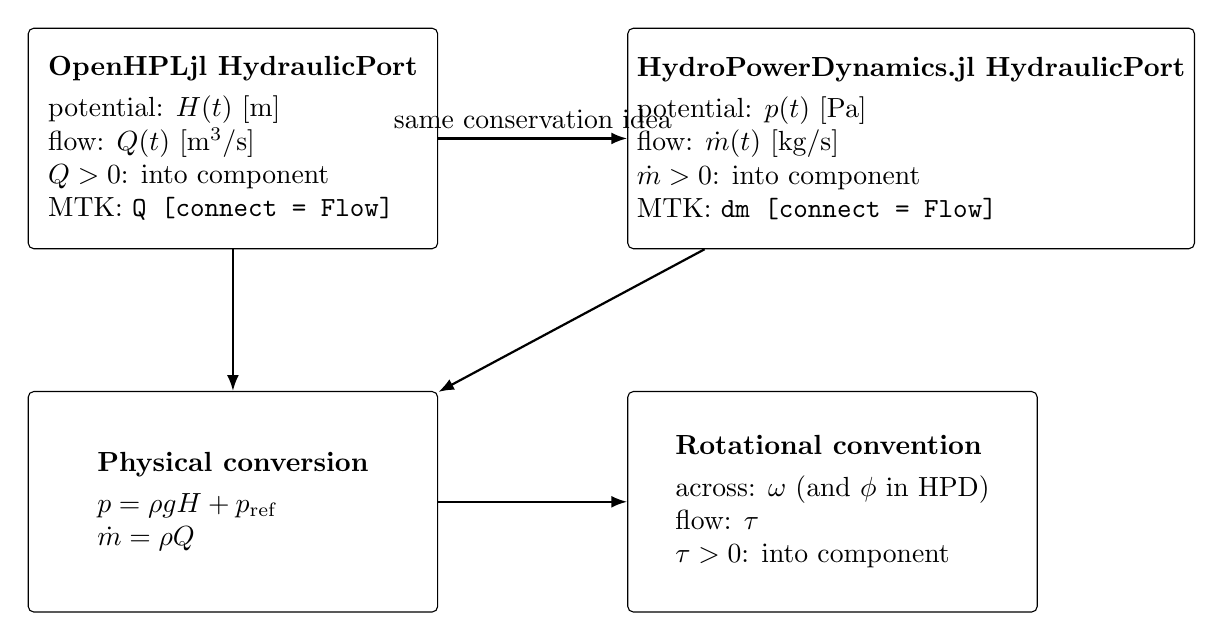
\begin{tikzpicture}[node distance=18mm and 24mm]
\node[box] (openh) {
\textbf{OpenHPLjl HydraulicPort}\\[1mm]
potential: $H(t)$ [m]\\
flow: $Q(t)$ [m$^3$/s]\\
$Q>0$: into component\\
MTK: \texttt{Q [connect = Flow]}
};

\node[box,right=of openh] (hpd) {
\textbf{HydroPowerDynamics.jl HydraulicPort}\\[1mm]
potential: $p(t)$ [Pa]\\
flow: $\dot m(t)$ [kg/s]\\
$\dot m>0$: into component\\
MTK: \texttt{dm [connect = Flow]}
};

\node[box,below=of openh] (conv) {
\textbf{Physical conversion}\\[1mm]
$p=\rho g H + p_{\rm ref}$\\
$\dot m=\rho Q$
};

\node[box,right=of conv] (rot) {
\textbf{Rotational convention}\\[1mm]
across: $\omega$ (and $\phi$ in HPD)\\
flow: $\tau$\\
$\tau>0$: into component
};

\draw[arr] (openh) -- node[above] {same conservation idea} (hpd);
\draw[arr] (openh) -- (conv);
\draw[arr] (hpd) -- (conv);
\draw[arr] (conv) -- (rot);
\end{tikzpicture}
\end{document}
